% Introduzione
\chapter{Introduzione}\label{ch:introduzione}
Il lavoro di tesi è stato realizzato in collaborazione con Magenta srl \cite{magenta} e con l'Istituto per la BioEconomia del Consiglio Nazionale delle Ricerche (IBE CNR) \cite{ibe}.\\

L'oggetto di studio è la piattaforma \textbf{AirQino} \cite{airqino} per il monitoraggio ambientale ad alta precisione in ambito urbano. Gli obiettivi sono stati molteplici:
\begin{itemize}
  \item Sviluppi tecnologici alla piattaforma, rivolti a migliorare in un caso l'affidabilità dei dati inviati dai sensori, e nell'altro la gestione del problema della quantità di dati in aumento costante (capitolo \ref{ch:sviluppi});
  \item Studio e analisi del processo di calibrazione delle centraline AirQino, con un confronto quantitativo sulle diverse tecniche utilizzate per la rilevazione di relazioni tra il segnale dei sensori e la stazione di riferimento (capitolo \ref{ch:calibrazione});
  \item Realizzazione di un'interfaccia che permetta la calibrazione di più centraline contemporaneamente  (capitolo \ref{ch:interfaccia}).
\end{itemize}

\begin{figure}[H]
\centering
\captionsetup{justification=centering}

\includegraphics[width=0.65\textwidth,height=\textheight,keepaspectratio]{img/magenta}
\caption{Magenta srl\\Fonte: \url{https://magentalab.it}}
\label{fig:magenta}
\end{figure}

\vspace{3mm}
\begin{figure}[H]
\centering
\captionsetup{justification=centering}

\includegraphics[width=0.85\textwidth,height=\textheight,keepaspectratio]{img/ibe.jpg}
\caption{CNR - Istituto per la BioEconomia (IBE)\\Fonte: \url{https://www.ibe.cnr.it}}
\label{fig:ibe}
\end{figure}

\vspace{3mm}
\begin{figure}[H]
\centering
\captionsetup{justification=centering}

\includegraphics[width=0.60\textwidth,height=\textheight,keepaspectratio]{img/airqino}
\caption{La piattaforma AirQino\\Fonte: \url{https://airqino.it}}
\label{fig:airqino}
\end{figure}

% Contesto
\section{Contesto}\label{sec:contesto}
Il monitoraggio della qualità dell'aria è una delle attività più importanti per la tutela della salute pubblica. La qualità dell'aria può essere influenzata da molte sorgenti di emissione di origine naturale e antropiche, tra cui le automobili, le centrali elettriche, gli impianti di riscaldamento e le fabbriche. Gli effetti dell'inquinamento atmosferico sulla salute sono molteplici e possono essere a breve o a lungo termine. In questo contesto, i dati raccolti dal monitoraggio della qualità dell'aria possono essere utilizzati per valutare l'impatto dell'inquinamento atmosferico sulla salute umana e sull'ambiente, e per identificare le principali fonti di inquinamento ambientale.

I principali inquinanti atmosferici sono l'ossido di zolfo (\ce{SO_{x}}), gli ossidi di azoto (\ce{NO_{x}}), il monossido di carbonio (\ce{CO}), l'ozono (\ce{O_{3}}) e il particolato atmosferico (\ce{PM} o polveri sottili). Per il particolato si parla di \ce{PM10} se le particelle hanno un diametro inferiore o uguale ai 10\textmu m, e \ce{PM_{2.5}} se inferiore o uguale ai 2.5\textmu m.

Il monitoraggio della qualità dell’aria è disciplinato in Italia dal DLgs. n. 155 del 13/08/2010, che recepisce la direttiva europea 2008/50/CE \cite{direttiva}. Il decreto assegna alle varie ARPA\footnote{Agenzia regionale per la protezione ambientale} regionali il compito istituzionale di effettuare il monitoraggio della qualità dell’aria e ne prescrive in dettaglio le modalità. Il monitoraggio viene effettuato attraverso stazioni ubicate in siti di campionamento sia fissi che mobili, in base a precisi criteri di esposizione: si distinguono quindi stazioni di fondo (urbane o suburbane), di traffico urbane, ed industriali. Ad esempio, nella città di Firenze la rete regionale di rilevamento gestita da ARPAT \cite{arpat} è costituita da 6 stazioni: 2 urbane-traffico, 3 urbane-fondo, ed una suburbana-fondo. Avendo valore normativo, le misure effettuate devono inoltre rispondere a precisi criteri di accuratezza ed essere sottoposte a precisi processi di validazione. \cite{relazione_alice}

Queste reti di monitoraggio sono quindi costituite da stazioni dotate di costose strumentazioni, oltretutto con elevati costi di manutenzione; un altro loro limite intrinseco è la rappresentatività strettamente puntuale delle misure (possono fornire misurazioni dettagliate e altamente accurate \cite{MEAD2013186}, ma soltanto in posizioni precise e sparse per una determinata città) \cite{s16050710}.
Questo rende difficile raccogliere informazioni rappresentative e affidabili per un'intera area urbana e, quindi, formare un quadro più chiaro sull'andamento dell'inquinamento. \cite{s16050710}

In questo scenario si inseriscono i nuovi sensori \textit{low-cost} per il monitoraggio dell’inquinamento atmosferico integrativo, soprattutto in situazioni in cui i sistemi di monitoraggio tradizionali risultano poco pratici \cite{doi:10.1021/es4022602}. Nell’acquisizione delle misure, infatti, i sensori di nuova generazione prevedono, a fronte di una minore accuratezza di misura, una serie di vantaggi quali: il basso costo di installazione, l'altra risoluzione temporale del dato acquisito e l'alta rappresentatività spaziale data dalla presenza capillare di più punti di acquisizione. \cite{relazione_alice}.
Oltre a fornire una rete più diffusa in grado di catturare efficacemente la variabilità dell'inquinamento atmosferico, il dispiegamento di sensori a basso costo in numero significativo può anche aiutare a valutare l'esposizione in tempo reale in modo da progettare strategie di mitigazione. \cite{KUMAR2015199}

La stessa direttiva europea 2008/50/CE \cite{direttiva} ha legittimato l’utilizzo di tali sensori, riconoscendo e regolamentando l’acquisizione di misure aggiuntive, anche a minor costo e minor precisione, ma che permettano di avere un quadro più completo (sia nello spazio che nel tempo) della qualità dell’aria. \cite{relazione_alice}

% Motivazioni
\section{Motivazioni}\label{sec:motivazoni}
Ci sono alcuni inconvenienti da tenere conto per quanto riguarda l'utilizzo di sensori a basso costo. Questi includono: 
\begin{itemize}
  \item Una minore accuratezza nelle misurazioni rispetto alle tradizionali stazioni di monitoraggio; \cite{s17112478}
  \item Sensibilità a fattori ambientali come temperatura, umidità e pressione;
  \item Derive del sensore, dovute all'usura dei componenti hardware, che richiedono frequenti ricalibrazioni \cite{s18092843};
\end{itemize}

La necessità di effettuare calibrazioni frequenti dei sensori implica la definizione di un \textbf{processo di calibrazione} che risulti il più possibile accurato ed efficiente. Inoltre alcuni tipi di sensori non forniscono output in unità ingeneristica, per cui la fase di calibrazione risulta obbligatoria.

Allo stesso tempo, un rete di monitoraggio ambientale deve fare i conti con la raccolta e l'analisi di grandi quantità di dati provenienti dai sensori in tempo reale. Su questo aspetto, uno degli obiettivi fondamentali per un sistema di questo tipo riguarda la necessità di garantire sempre \textbf{affidabilità} e \textbf{disponibilità} dei dati. Inoltre, dal punto di vista tecnologico si deve prevedere l'utilizzo di soluzioni che permettano al sistema di \textbf{scalare} facilmente in caso di crescita del numero di stazioni e di sensori. In generale si tratta di problemi difficili da affrontare, sia per quantità di dati che per affidabilità.

Il lavoro svolto si colloca proprio in questo contesto, con il duplice obiettivo di (i) studiare, analizzare e confrontare soluzioni diverse per il processo di calibrazione di centraline e (ii) aumentare sia la scalabilità del sistema che l'affidabilità e la disponibilità dei dati inviati dai sensori.

% La piattaforma AirQino
\section{La piattaforma AirQino}\label{sec:airqino}
AirQino è una piattaforma di monitoraggio ambientale ad alta precisione, realizzata dal Consiglio Nazionale delle Ricerche (CNR) in collaborazione con TEA Group e Quanta Srl. \cite{GUALTIERI2017609}
Il progetto nasce dall’esigenza di realizzare una rete di stazioni mobile per un monitoraggio più completo della qualità dell’aria in ambito urbano, in linea con la direttiva europea 2008/50/EC \cite{direttiva}, che riconosce e regolamenta l’importanza di misure aggiuntive rispetto a quelle delle stazioni fisse. 

Alcune delle caratteristiche di AirQino sono:

\begin{itemize}
  \item Sistema di rilevamento \textbf{polifunzionale}: il sistema offre la possibilità di rilevare gli agenti inquinanti presenti in atmosfera;
  \item Sistema \textbf{versatile} e dispiegabile in più punti per creare una rete di monitoraggio capillare, flessibile ed economica;
  \item Alte \textbf{prestazioni} dei sensori installati, garantite da una rigorosa calibrazione e validazione degli apparati da parte dei laboratori del CNR;
  \item Tutte le stazioni sono \textbf{configurabili} con un’ampia gamma di sensori aggiuntivi a seconda delle proprie esigenze. \cite{airqino}
\end{itemize}

La rete di sensori AirQino consente rilevare le principali sostanze inquinanti riscontrabili nell’aria (\ce{NO2}, \ce{O3}, \ce{CO}, \ce{PM_{2.5}}, \ce{PM_{10}}) ma anche ulteriori parametri ambientali, come la temperatura, l'umidità relativa dell’aria e il principale gas climalterante, la \ce{CO2}.
Inoltre la centralina è \textbf{estendibile}, e permette di aggiungere ulteriori sensori ausiliari in base alle necessità.

\begin{figure}[H]
\centering
\captionsetup{justification=centering}
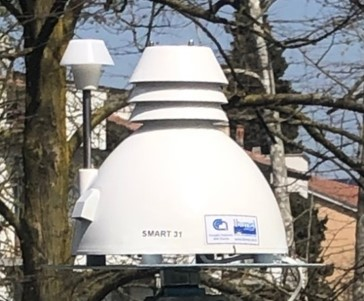
\includegraphics[width=0.60\textwidth,height=\textheight,keepaspectratio]{img/airqino_stazione}
\caption{Una centralina AirQino\\Fonte: \url{https://airqino.it}}
\label{fig:airqino_stazione}
\end{figure}

\begin{figure}[H]
\centering
\captionsetup{justification=centering}
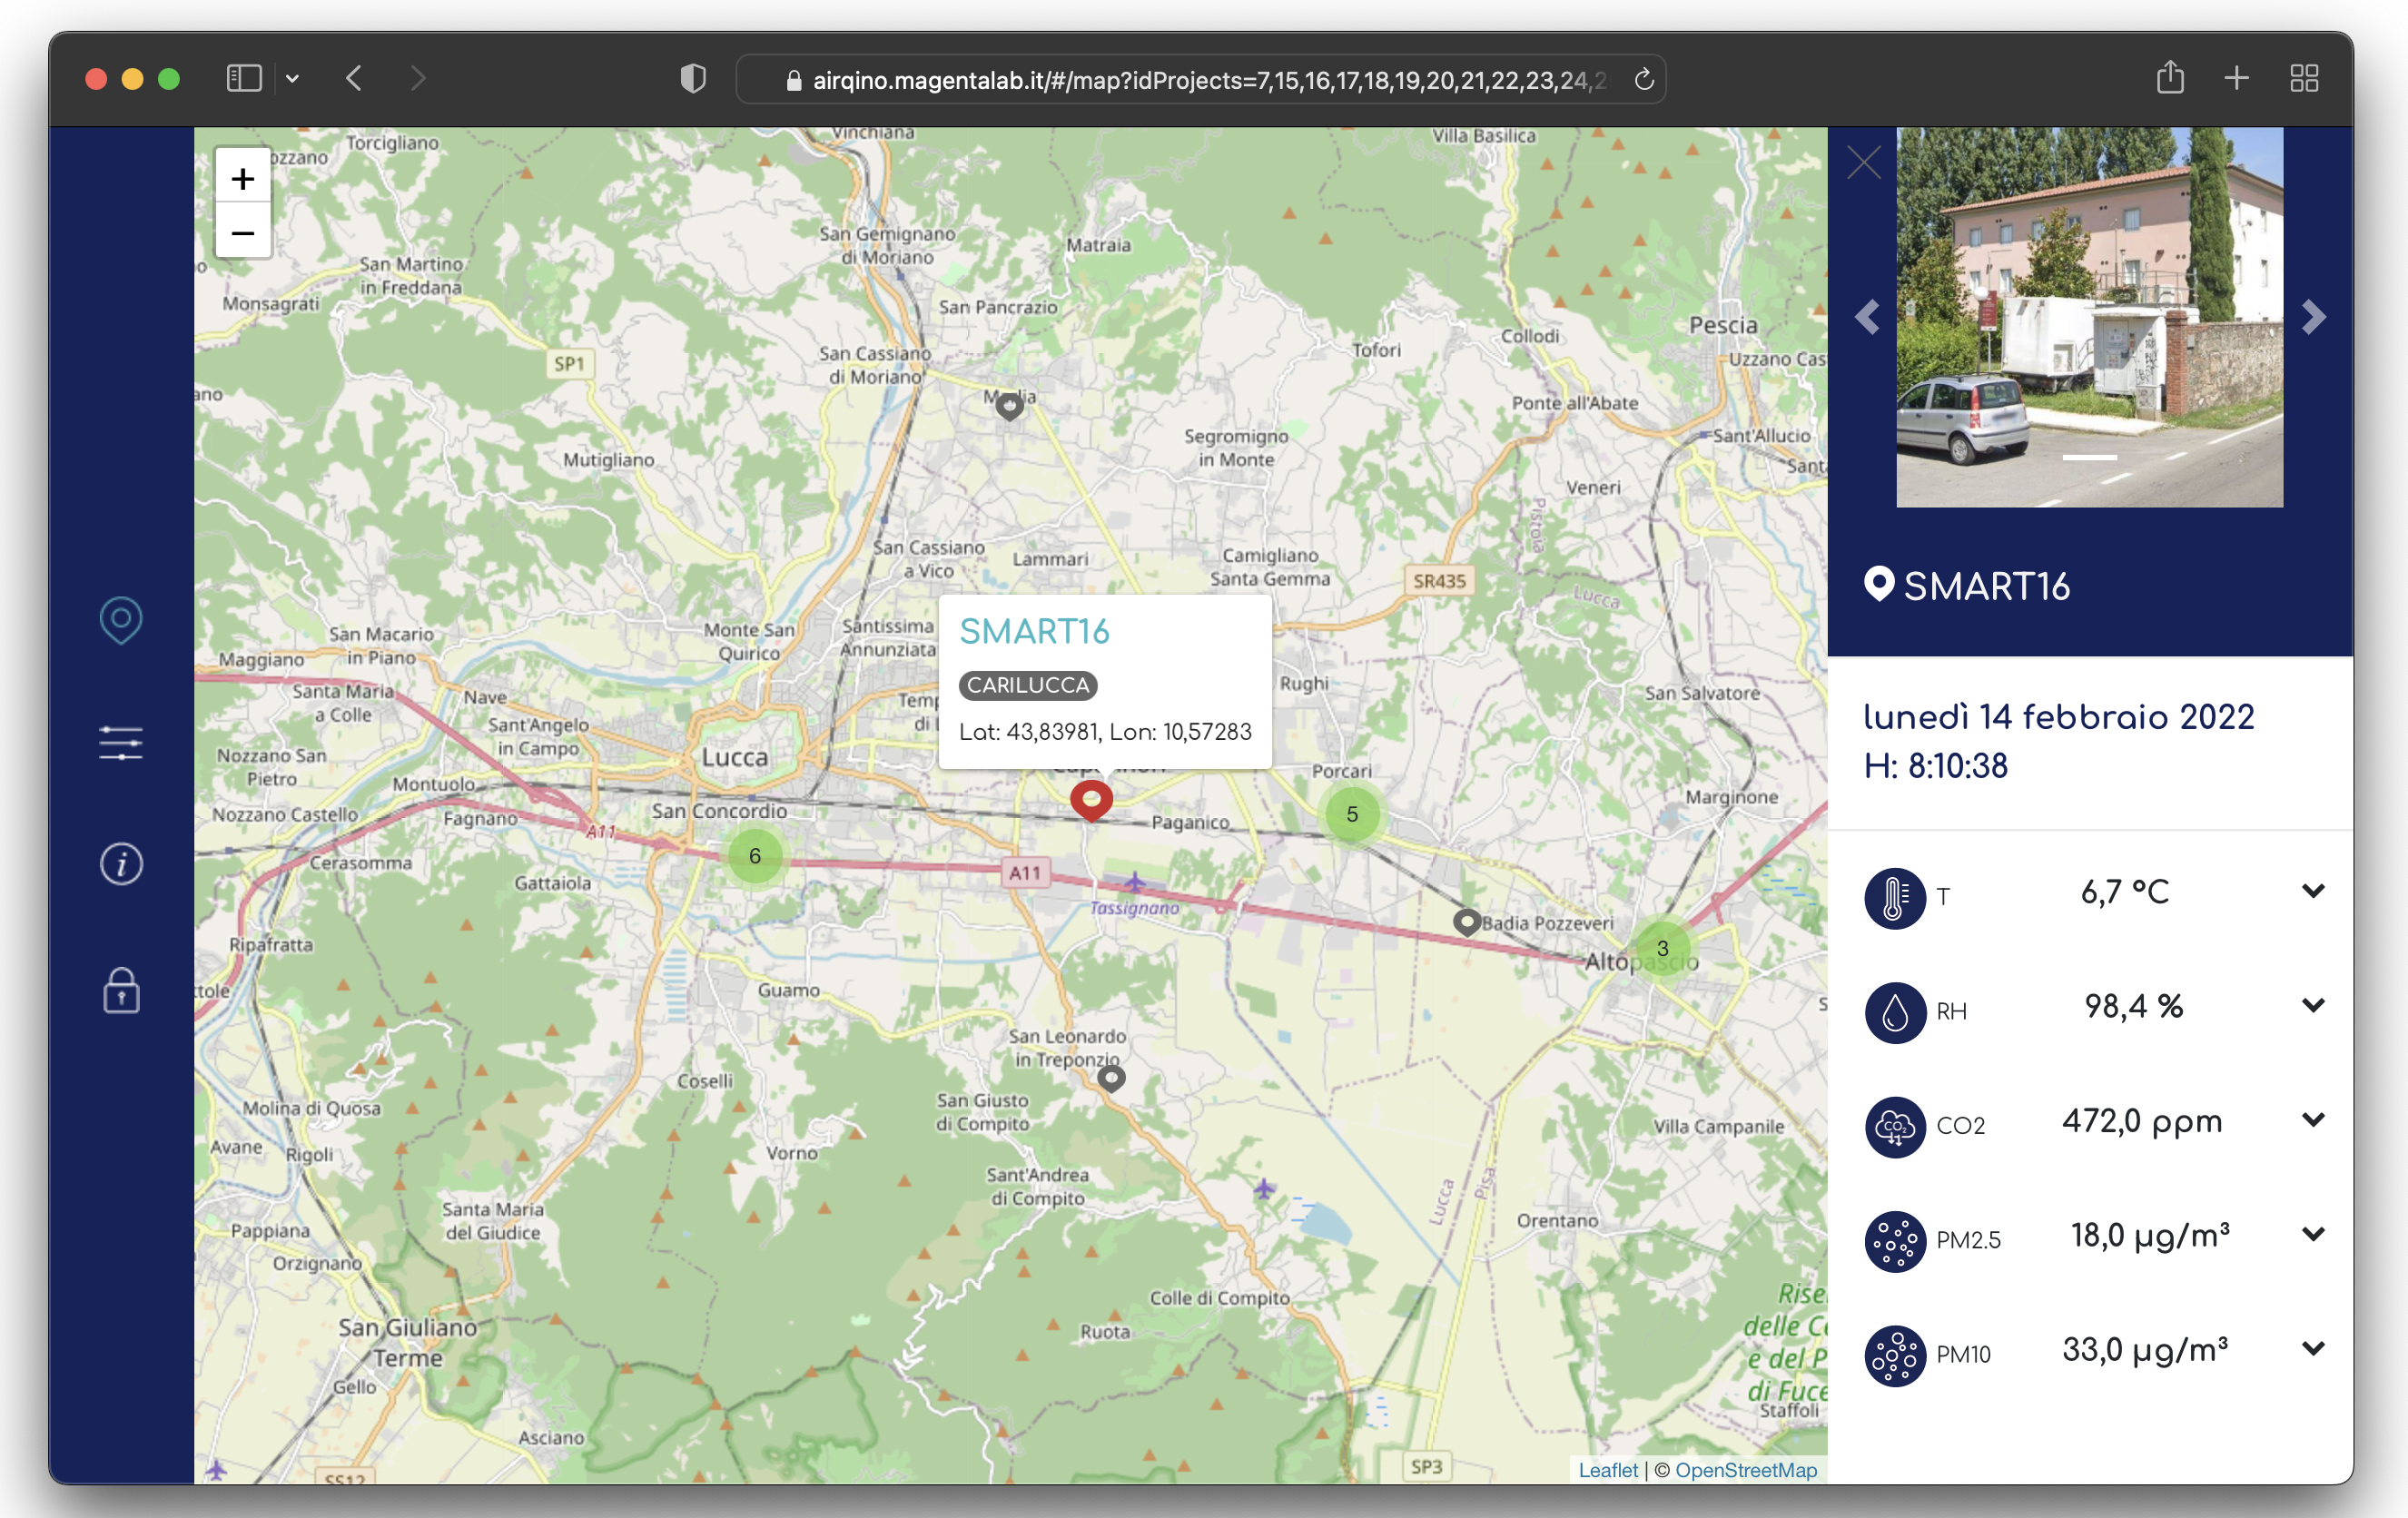
\includegraphics[width=0.80\textwidth,height=\textheight,keepaspectratio]{img/airqino_web}
\caption{La piattaforma web di AirQino\\Fonte: \url{https://airqino.magentalab.it}}
\label{fig:airqino_web}
\end{figure}

\clearpage

La piattaforma AirQino mette inoltre a disposizione un portale web per la consultazione dei dati, all'indirizzo \url{https://airqino.magentalab.it}. 

La piattaforma consiste in una mappa interattiva che visualizza tutte le reti di centraline. Selezionata una stazione di interesse, vengono mostrati dettagli e foto della stazione stessa (figura \ref{fig:airqino_web}). Per ciascun sensore della centralina selezionata è possibile visualizzare grafici di andamento medio settimanali, insieme al dato istantaneo relativo all'ultima misurazione, nell'unità di misura come da normativa. \cite{airqino}

\subsection{Architettura e tecnologie}\label{ssec:airqino-architettura}
L'architettura del sistema AirQino è organizzata nei seguenti elementi principali (\ref{fig:airqino-arch}):

\begin{itemize}
  \item \textbf{Gateway}: server che espone servizi compatibili con le centraline, e normalizza i dati trasmessi verso il server di raccolta. Questa applicazione, realizzata con Java e framework \textbf{Spring} \cite{spring}, fornisce un endpoint con lo stesso indirizzo a cui le centraline comunicano, in modo da garantire continuità di servizio. Il gateway ha anche il compito di segnalare eventuali interruzioni di funzionamento, secondo regole ben definite. Il gateway produce anche un output su protocollo \textit{MQTT2}, utilizzando un broker open source per pubblicare i dati verso il backend;
  \item \textbf{Backend}: applicazione server che si interfaccia con il broker \textit{MQTT} e scrive sul database i dati, esponendo inoltre servizi web di tipo REST utilizzati dal frontend web. Il backend è realizzato con Java e framework \textbf{Spring} \cite{spring} e utilizza \textbf{Timescale} \cite{timescale}, un database relazionale open source per la gestione efficienti di dati temporali;
  \item \textbf{Frontend}: applicazione web che permette la visualizzazione di mappa e grafici dei dati raccolti dalle centraline, utilizzando i servizi esposti dal backend. L'interfaccia è basata su tecnologia \textbf{Angular} \cite{angular}. Il frontend ha anche una sezione \textit{admin}, protetta da autenticazione, che permette la gestione del sistema. Le funzionalità di gestione previste sono:
    \begin{itemize}
      \item Gestione anagrafica centraline (nome, posizione, progetti a cui afferisce);
      \item Configurazione dei parametri di funzionamento, tra cui i parametri di calibrazione (per la trasformazione da dati grezzi a valori leggibili dall’utente) e le soglie di rilevamento allarmi;
      \item Gestione utenti;
      \item Scaricamento di dati raw oppure calibrati. \cite{airqino}
    \end{itemize}
\end{itemize}

\begin{figure}[H]
\centering
\captionsetup{justification=centering}
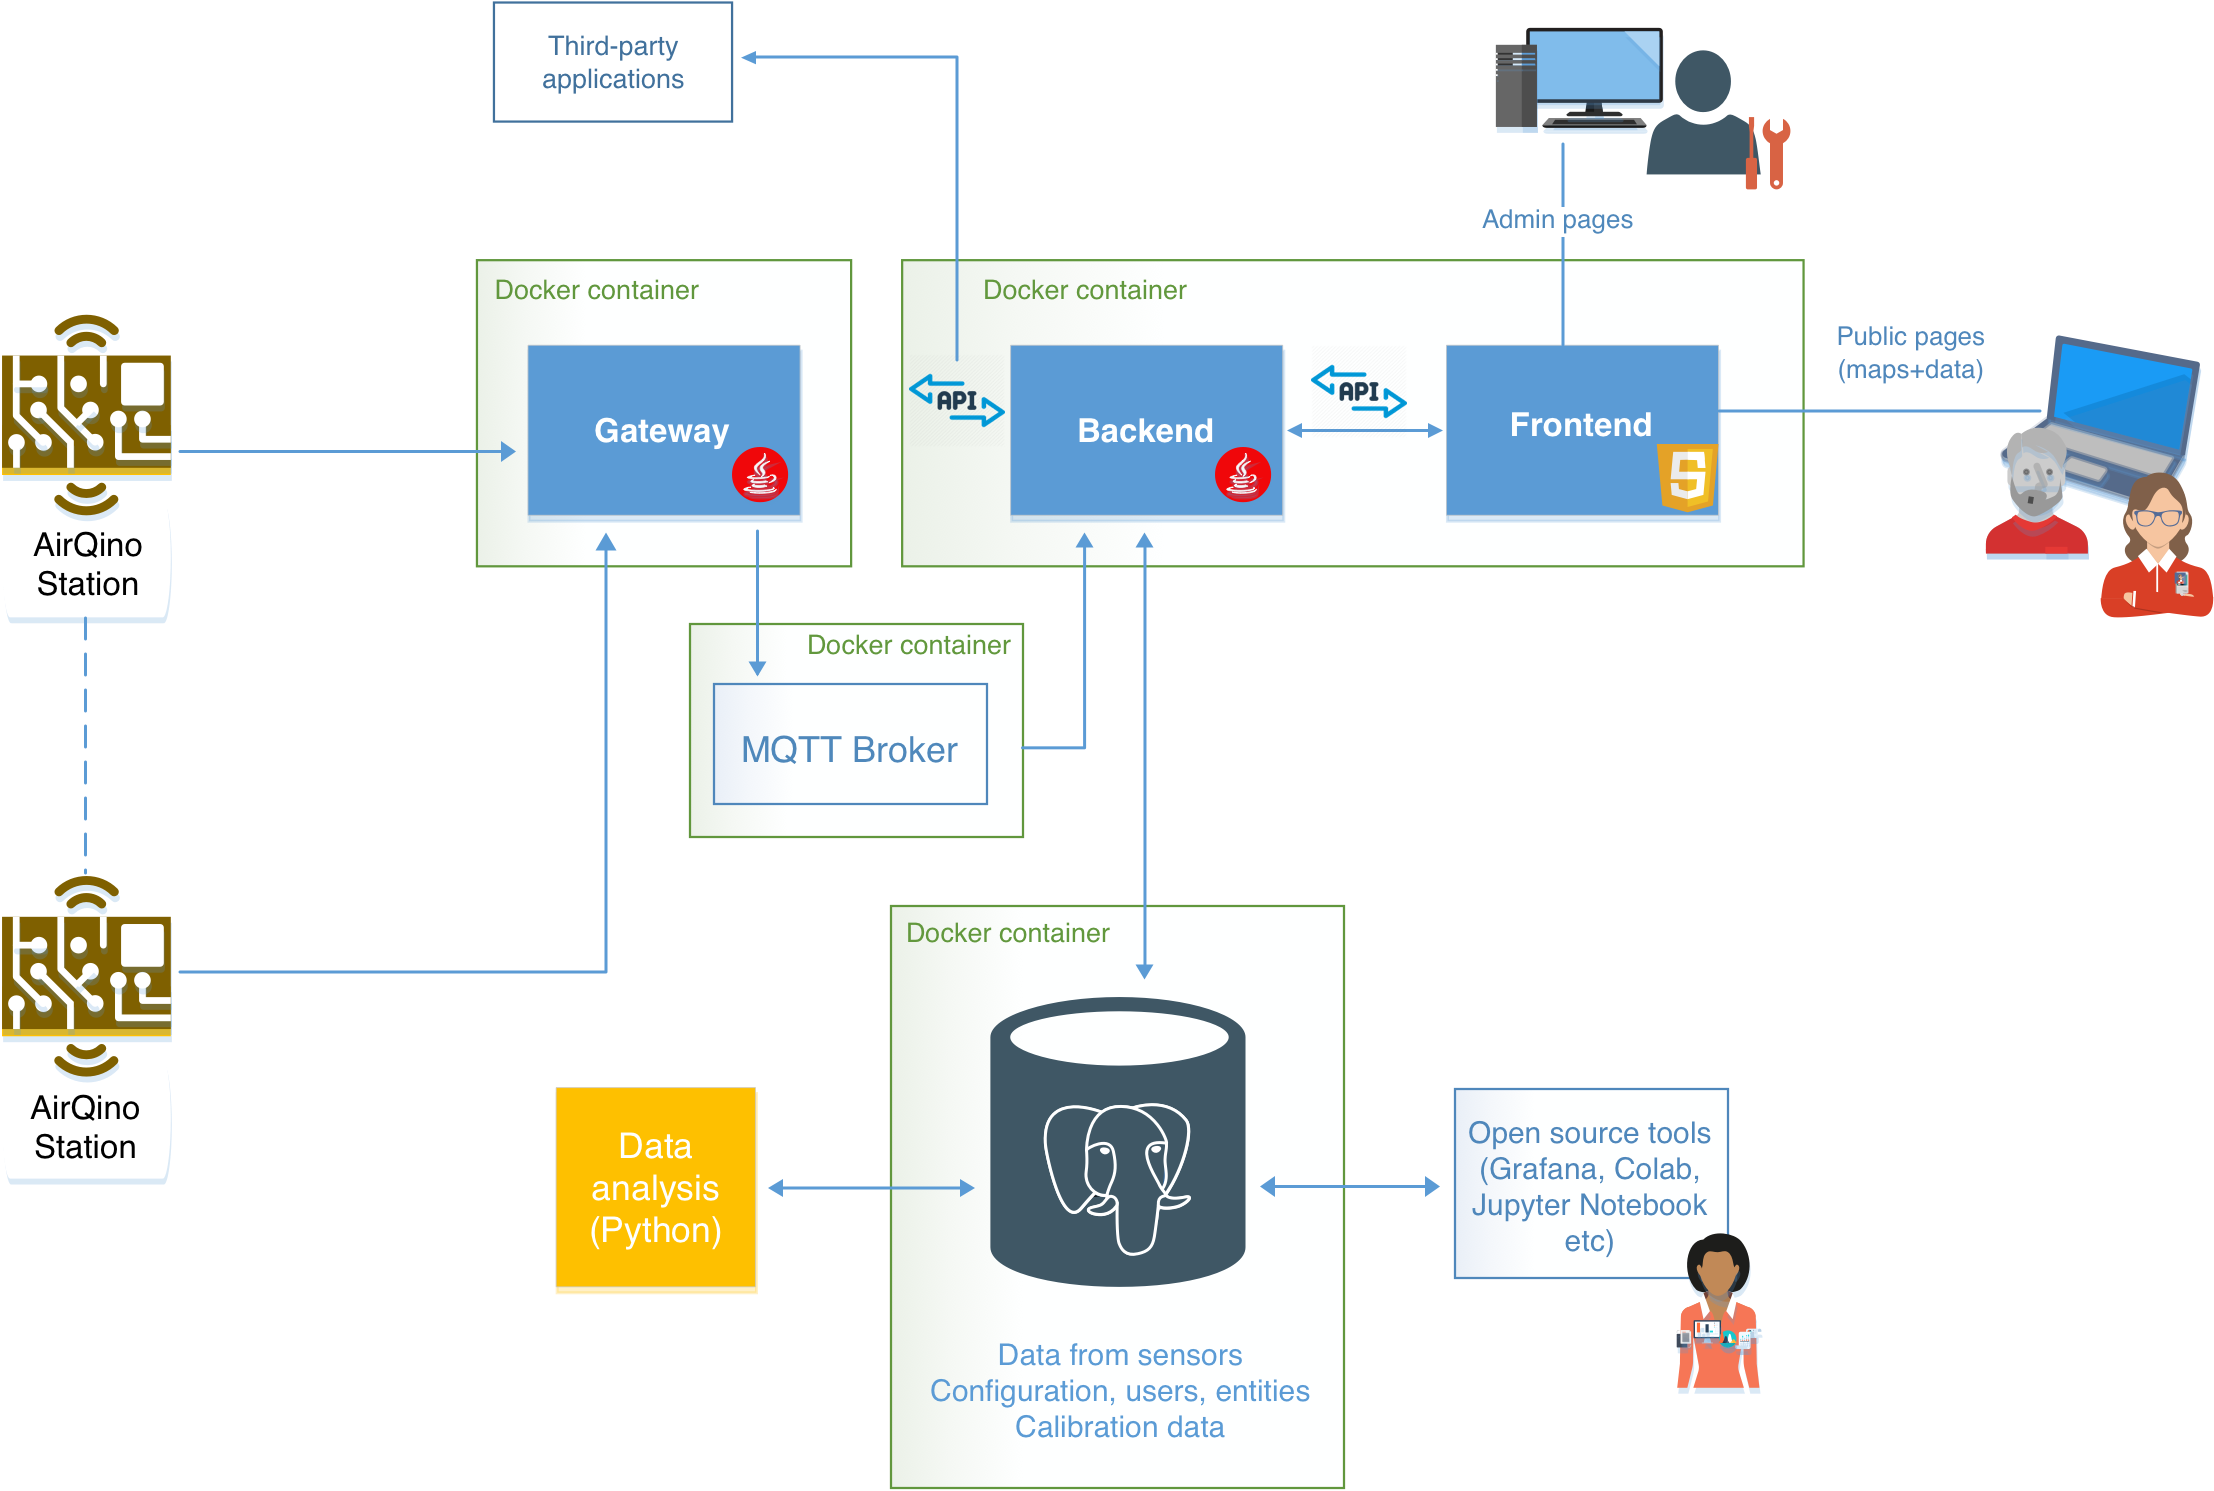
\includegraphics[width=0.85\textwidth,height=\textheight,keepaspectratio]{img/airqino_arch}
\caption{Schema architetturale della piattaforma AirQino}
\label{fig:airqino-arch}
\end{figure}

% Sensori
\subsection{Sensori}\label{ssec:hardware}
La tabella \ref{fig:sensori-airqino} mostra le varie tipologie di sensori che sono in dotazione con le centraline AirQino, con il rispettivo principio di funzionamento, range e precisione.

\begin{table}[H]
    \footnotesize
    \centering
    \def\arraystretch{0.9}
    \begin{tabular}{|l|l|l|l|l|l|}
    \hline
        \textbf{Sensori} & \textbf{Tipologia} & \textbf{Unità} & \textbf{Range} & \textbf{Prec.} \\ \hline
        \ce{NO2} & Sensori di gas MOS & $\mathrm{\si{\micro}g/m^3}$ & 0-5000 & 15\% \\ \hline
        \ce{O3} & Semiconduttore & $\mathrm{\si{\micro}g/m^3}$ & 0-1000 & 15\% \\ \hline
        CO & Sensori di gas MOS & $\mathrm{\si{\micro}g/m^3}$ & 0-30 & 15\% \\ \hline
        VOC totali & Sensori di gas MOS & $\mathrm{\si{\micro}g/m^3}$ & 0-1000 & 15\% \\ \hline
        \ce{CO2} & NDIR & ppm & 0-2000 & 10\% \\ \hline
        \ce{PM_{2.5}} & Contatore di particelle ottico & $\mathrm{\si{\micro}g/m^3}$ & 0-1000 & 10\% \\ \hline
        \ce{PM10} & Contatore di particelle ottico & $\mathrm{\si{\micro}g/m^3}$ & 0-1000 & 10\% \\ \hline
        Umidità relativa & Stato solido & \% & 0-100 & 5\% \\ \hline
        Temp. dell’aria & Stato solido & °C & -40 - 80 & 5\% \\ \hline
        Temp. interna & Stato solido & °C & -40 - 80 & 5\% \\ \hline
    \end{tabular}
    \captionsetup{justification=centering}
    \caption{Tipologie di sensori in dotazione con le centraline AirQino (configurazione base, estendibile). Fonte: \url{https://airqino.it}}
    \label{fig:sensori-airqino}
\end{table}

Nello specifico i sensori utilizzati sono:
\begin{itemize}
  \item \textbf{SenseAir S8} per acquisizione \ce{CO2};
  \item \textbf{DHT22} per umidità relativa e temperatura;
  \item \textbf{MiCS-2614} per \ce{O3};
  \item \textbf{MiCS-2714} per \ce{NO2};
  \item \textbf{TGS-2600} per \ce{VOC};
  \item \textbf{SDS011} per \ce{PM_{2.5}} e \ce{PM10}. \cite{relazione_alice}
\end{itemize}

Oggetto di questo studio sono stati due sensori con principi di funzionamento diversi: MiCS-2714 (\ref{sensore-no2}) per \ce{NO2} e SDS011 (\ref{sensore-pm}) per \ce{PM_{2.5}} e \ce{PM_10}.

\subsubsection{MiCS-2714}\label{sensore-no2}
Il MiCS-2714 è un sensore di tipo MOS, ovvero costituito da un \textit{film} depositato su una piastra di elementi riscaldanti la cui temperatura operativa è generalmente compresa tra 300°C e 500°C. \cite{relazione_alice}

\begin{figure}[H]%
    \centering
    \captionsetup{justification=centering}
    \subfloat[\centering Foto del sensore]{{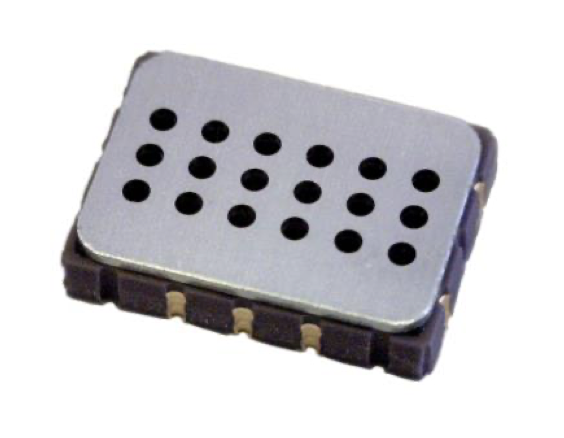
\includegraphics[width=6.7cm]{img/mics1} }}%
    \subfloat[\centering Circuito]{{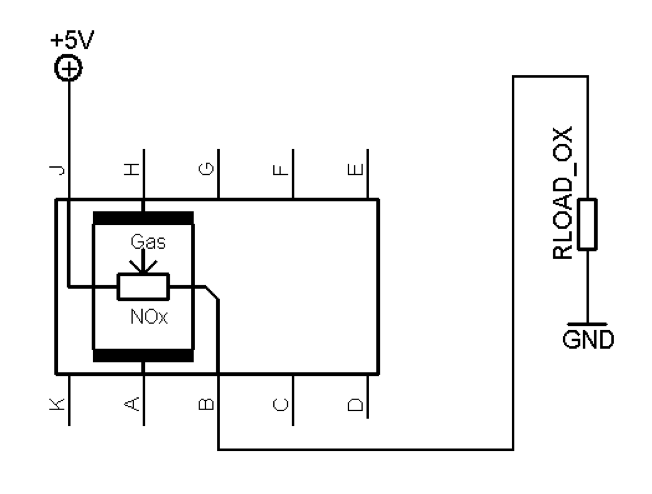
\includegraphics[width=6.4cm]{img/mics2} }}%
    \caption{Il sensore MiCS-2714 per il rilevamento di \ce{NO2}\\Fonte: \url{https://mouser.it}}%
    \label{fig:mics}%
\end{figure}

Di solito il  materiale funzionale del \textit{film} più adatto per la rilevazione di \ce{NO2} è l’ossido  di  ferro e lantanio (\ce{LaFeO3}), che oltre ad avere una buona sensibilità agli ossidi di azoto ha una bassa sensibilità al  monossido di carbonio. Questo tipo  di  materiale  funzionale risulta  molto  sensibile  ai  gas  ossidanti, come \ce{O3} e \ce{NO2}. 
Qualsiasi sia il materiale funzionale, il principio di funzionamento per tutti i MOS nella rilevazione di gas è quello di interagire con il gas presente all’interno dell’atmosfera tramite reazioni di ossidoriduzione, portando a un cambiamento di conduttività, che viene rilevato da un circuito apposito. Le variazioni della conduttività dei sensori è fortemente influenzata dalle variazioni di umidità e temperatura \cite{relazione_alice}. Di seguito le specifiche del sensore MiCS-2714 come riportate dal \textit{datasheet}:

\begin{table}[H]
    \footnotesize
    \centering
    \begin{tabular}{|l|l|}
    \hline
        \textbf{Parametro} & \textbf{Specifica} \\ \hline
        \textbf{Range di misura} & 0.05 – 10ppm \\ \hline
        \textbf{Tensione di alimentazione} & 4.9-5.1V \\ \hline
        \textbf{Ciclo di vita} & >2 anni \\ \hline
        \textbf{Dimensioni} & 12×16mm \\ \hline
        \textbf{Peso} & 4g \\ \hline
    \end{tabular}
    \captionsetup{justification=centering}
    \caption{Specifiche tecniche del sensore MiCS-2714\\Fonte: \url{https://mouser.it}}
    \label{fig:mics-specifiche}
\end{table}

\subsubsection{SDS011}\label{sensore-pm}
Il sensore SDS011 basa il suo funzionamento sul principio della diffusione ottica (detta anche dispersione o \textit{scattering}). In particolare, un raggio luminoso che procede in una certa direzione, quando colpisce una particella, viene diffuso in maniera disordinata in tutte le direzioni. \cite{sds}

\begin{figure}[H]%
    \centering
    \captionsetup{justification=centering}
    \subfloat[\centering Foto del sensore]{{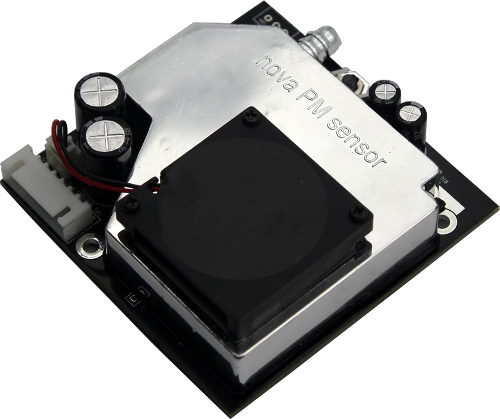
\includegraphics[width=5.3cm]{img/sds1} }}%
    \subfloat[\centering Componenti interni]{{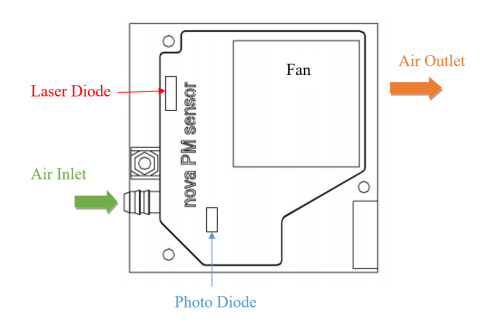
\includegraphics[width=6.8cm]{img/sds2} }}%
    \caption{Il sensore SDS011 per il rilevamento di \ce{PM_{2.5}} e \ce{PM10}\\Fonte: \url{https://circuitdigest.com}}%
    \label{fig:mics}%
\end{figure}

Il sensore è costituito da una ventola che aspira l’aria esterna per convogliarla in una camera di misura stagna. All’interno della camera di misura è contenuto un diodo laser e un fotodiodo rilevatore (figura \ref{fig:mics} (b)). Appena l’aria viene immessa nella camera, il laser viene acceso: un fascio di luce laser procede “dritto” senza diffondersi. Quando il laser colpisce il particolato, la sua luce viene diffusa e l’intensità luminosa che si disperde nella camera può essere rilevata dal fotodiodo. 
Il sensore riesce a distinguere tra il \ce{PM10} e il \ce{PM_{2.5}} perché la forma d’onda della luce rilevata dal fotodiodo è correlata con il numero e le dimensioni delle particelle: per questo motivo a bordo del sensore c’è un microcontrollore ad 8 bit che esegue l’analisi \cite{sds}.
Di seguito le specifiche del sensore SDS011 come riportate dal \textit{datasheet}:

\begin{table}[H]
    \footnotesize
    \centering
    \begin{tabular}{|l|l|}
    \hline
        \textbf{Parametro} & \textbf{Specifica} \\ \hline
        \textbf{Range di misura} & 0-1000 $\mathrm{\si{\micro}g/m^3}$ \\ \hline
        \textbf{Tensione di alimentazione} & 4.7-5.3V \\ \hline
        \textbf{Ciclo di vita} & 11 mesi \\ \hline
        \textbf{Dimensioni} & 71×70mm \\ \hline
        \textbf{Peso} & 6g \\ \hline
    \end{tabular}
    \captionsetup{justification=centering}
    \caption{Specifiche tecniche del sensore SDS011\\Fonte: \url{https://reichelt.com}}
    \label{fig:sds-specifiche}
\end{table}

\subsection{Progetti che includono la piattaforma AirQino}\label{ssec:correlati}
Di seguito sono elencati alcuni progetti che fanno uso delle centraline AirQino:

\begin{itemize}
  \item \textbf{Prato Urban Jungle} \cite{urbanjungle} mira a promuovere la progettazione urbana creativa e visionaria per ri-naturalizzare i quartieri di Prato in modo sostenibile e socialmente inclusivo;
  \item \textbf{SMART Treedom} \cite{smartreedom} è il frutto dalla collaborazione tra Treedom e l’Istituto di Biometeorologia del Consiglio Nazionale delle Ricerche. La finalità del progetto è stata quella di prototipare un sistema integrato che possa essere modulato con diversi sensori in base al tipo di grandezza fisica che si vuole misurare e una tecnologia laser per la misura delle polveri sottili;
  \item \textbf{Trafair} \cite{trafair} è un progetto europeo biennale co-finanziato dal programma europeo Connecting Europe Facility (CEF) nel settore delle telecomunicazioni con lo scopo di sviluppare un servizio di previsione della qualità dell’aria urbana basata su previsioni meteo e flussi di traffico in sei città europee di dimensioni diverse: Zaragoza, Firenze, Modena, Livorno, Santiago de Compostela e Pisa;
  \item \textbf{Smart Garda Lake} \cite{garda} nasce nel 2017 con lo scopo di creare una rete di monitoraggio ambientale per rilevamenti in campo meteorologico, inquinamento acustico, stato delle acque superficiali e qualità dell’aria all’insegna degli obiettivi di sostenibilità dell’Agenda 2030 dell’ONU;
  \item \textbf{PlanetWatch} \cite{planetwatch} è una piattaforma decentralizzata che consente di monitorare e proteggere il pianeta attraverso la condivisione di informazioni. Gli utenti possono condividere informazioni sull'ambiente, la sostenibilità e la responsabilità sociale;
  \item \textbf{Brenner LEC} \cite{lec} si colloca nel contesto di un’area sensibile come le Alpi e si pone l’obiettivo di creare un “corridoio a emissioni ridotte” (LEC – Lower Emission Corridor) lungo l’asse autostradale del Brennero al fine di ottenere un chiaro beneficio ambientale nei settori della tutela dell’aria e della protezione del clima, nonché una riduzione dell’inquinamento acustico.
\end{itemize}

\subsection{Altre piattaforme}\label{ssec:competitor}
Esistono anche altre piattaforme con obiettivi simili ad AirQino:

\begin{itemize}
	\item \textbf{Airly} \cite{airly} è una piattaforma che consente di condividere informazioni ambientali in tempo reale, grazie alla quale è possibile monitorare la qualità dell'aria e i livelli di inquinamento;
	\item \textbf{Aqicn} \cite{aqicn} è un progetto open source lanciato nel 2010 che consente di monitorare l'inquinamento atmosferico in tempo reale;
	\item \textbf{IQAir} \cite{iqair} è una società svizzera che produce e vende purificatori d'aria per uso residenziale e commerciale. La loro applicazione fornisce un rapporto in tempo reale sulla qualità dell'aria e previsione dell'inquinamento atmosferico;
	\item \textbf{Decentlab} \cite{decentlab} è un'azienda svizzera che fornisce dispositivi e servizi di sensori wireless per soluzioni di monitoraggio distribuite ed economiche;
	\item \textbf{HackAIR} \cite{hackair} è una piattaforma open source che consente ai cittadini di monitorare la qualità dell'aria nei propri quartieri. Gli utenti possono interagire con la piattaforma per segnalare la qualità dell'aria nel proprio quartiere, visualizzare i dati relativi alla qualità dell'aria e condividere informazioni e dati con altri utenti.
\end{itemize}
